


\documentclass{article}

\usepackage[romanian]{babel}
\usepackage{graphicx}
\usepackage{hyperref}
\usepackage{tikz}
\usepackage{pgfplots}




\author{Eduard-Mihail Hamza}
\title{Comparație experimentală între un Algoritm Genetic și metodele Hill Climbing și Simulated Annealing pentru optimizarea unor funcții cu număr variabil de parametri}

\begin{document}
\maketitle

\section{Introducere}

În analiza matematică, maximul și minimul unei funcții sunt cele mai mari, respectiv cele mai mici valori, pe care funcția le poate lua, fie pe un anume interval (caz în care poartă denumirea de maxim/minim local) sau pe întreg domeniul de definiție al funcției (caz în care se numește maxim/minim global).\\ \\
În acest raport se va realiza o comparație între un \textbf{algoritm genetic de optimizare} și metodele \textbf{Hill Climbing} și \textbf{Simulated Annealing} și se vor prezenta câteva date experimentale ce caracterizază execuția acestor algoritmi de aflare a minimului global al unei funcții cu număr variabil de parametri.

 
\subsection{Motivație}
Problemele de optimizare a unei funcții presupun gasirea minimului sau maximului unei funcții pe un interval. Astfel de probleme se abordează de obicei, atunci când instrumentele matematice clasice nu mai pot oferii soluții, cu ajutorul algoritmilor genetici. Una dintre cele mai mari provocări ale acestor algoritmi de optimizare este găsirea minimului/maximului global fără a rămâne blocați in minime/maxime locale.\\
Acest raport își propune să observe care dintre cele trei metode amintite mai sus are rezultate mai bune în funcție de fiecare funcție de test în parte și în funcție de dimensiunea fiecărei funcții.

\section{Metode}
Implementarea \textbf{algoritmului genetic} s-a realizat dupa o schmeă clasică în care se generează o populație inițială care apoi evoluează de-a lungul mai multor generații (prin crossovere și mutații) sub controlul unei funcții fitness care măsoară meritul individual.\\
Mai jos sunt amintite câteva detalii de implementare:
\begin{itemize}
\item Număr generații: $1000$
\item Probabilitate mutație: $0.001$
\item Probabilitate crossover: $0.4$
\item Monstră statistică: $30$
\end{itemize}
În ceea ce privește metoda de selecție a fost folosită \textbf{roata norocului}, metodă prin care numărul estimat de copii pe care îl primește un individ este proporțional cu fitness-ul său împărțit la fitness-ul total al populației.\\ \\
Mai jos este prezentat codul \textbf{funcței fitness} folosită: 
\begin{verbatim}
def fitness(individ, fct):
    global dimension

    Epsilon = 0.1
    result = fct(decode(individ))

    if fct == Schwefel:
        result = result + 418.9829 * dimension

    if fct == Michalewicz:
        result = -1 * result

    fitness_value = 1 / (result + Epsilon)

    return fitness_value
    
    
\end{verbatim}
Celelalte 2 metode folosite au fost \textbf{Hill Climbing} și \textbf{Simulated Annealing}:\\
\textbf{Hill Climbing}, o metodă iterativă ce realizează o căutare locală. Este utilizată varianta iterată (Iterated Hill Climbing) în care HC este restartat, pentru a mări gradul de explorare a spațiului de căutare.\\
De asemenea, se vor folosii 2 tipuri de HC:  \textbf{Best Improvment Hill Climbing} și \textbf{First Improvment Hill Climbing}.\\
\textbf{Best Improvment Hill Climbing} examinează fiecare vecin și îl alege pe cel care determină cea mai bună soluție.\\
\textbf{First Improvment Hill Climbing} nu examinează fiecare vecin înainte de a hotărî pe care îl alege. Pur și simplu alege un vecin la întâmplare pâna când găsește unul mai promițător decât cel curent.\\
\textbf{Simulated Annealing}, o meta-euristtică de tip traiectorie care permite o mai bună explorare a spațiului 
și ieșirea din puncte de optim local, dând posibilitatea vizitării unor soluții de calitate mai slabă decât cea curentă. \\
Pentru funcția de modificare a temperaturii s-a folosit înmultirea cu un numar subunitar (0.9), aceasta fiind inițializata la începutul algoritmului cu valoarea 1000.\\
În cazul tuturor metodelor pentru \textbf{reprezentarea soluțiilor} s-au folosit șiruri de biti, iar \textbf{precizia} utilizată a fost $10^{-2}$ (2 zecimale).

\section{Experiment}
Pentru testarea algoritmilor vom folosi următoarele funcții:
\begin{enumerate}
\item \textbf{Functia lui De Jong 1}
$$ f(x) = \sum_{i=1}^n x_i^2, 
x_i \in \left[ -5.12, 5.12 \right]$$

\includegraphics[scale=0.5]{spheref.png}

Minim global: 0

\item \textbf{Functia lui Schwefel}
$$ f(x) = \sum_{i=1}^n -x_i \cdot \sin (\sqrt{\mid x_i\mid}),
x_i \in \left[ -500, 500\right]  $$

\includegraphics[scale=0.5]{schwef.png}

Minim global: $-n \cdot 418.9829$
\item \textbf{Functia lui Rastrigin}
$$ f(x) = A \cdot n + \sum_{i=1}^n \left[ x_i^2 - A \cdot cos(2 \pi x_i) \right],
A = 10, x_i \in \left[ -5.12, 5.15 \right]$$

\includegraphics[scale=0.5]{rastr.png}

Minim global: 0
\item \textbf{Functia lui Michalewicz}
$$ f(x) = -\sum_{i=1}^n \sin (x_i) \cdot \left( \sin \left( \frac{i \cdot x_i^{2}}{\pi} \right) \right)  ^{2m},
m = 10, x_i \in \left[ 0, \pi \right] $$

\includegraphics[scale=0.5]{michal.png}

Minim global: -4.687 (n=5), -9.66 (n=10)
\end{enumerate}


\section{Rezultate}
teoretic = minimul teoretic al funcției (cel corect)\\\
minim = cel mai bun minim returnat de algoritm\\
medie = media minimelor obținute\\
$\sigma$ = deviație standard\\
timp = timpul mediu de execuție în secunde\\
GA = algoritm genetic\\
BIHC = Best Improvment Hill Climbing\\
FIHC = First Improvment Hill Climbing\\
SA = Simulated Annealing


\clearpage
\subsection{5 dimensiuni}

\begin{figure}[!h]
\begin{tabular}{||c|||l|l|l|l||}
  \hline
  \multicolumn{5}{||c||}{Rastrigin (teoretic min=0)} \\ \hline
  Algoritm & minim & medie & $\sigma$ & timp(s) \\ \hline \hline
  GA & 0.02 & 2.80 & 1.65 & 8.273 \\ \hline
  BIHC & 0.02 & 1.53 & 0.72 & 2.474\\ \hline
  FIHC & 0.02 & 2.04 & 1.25 & 0.475 \\ \hline
  SA & 1.01 & 6.12 & 3.49 & 0.527 \\ \hline
\end{tabular}
\caption{Rastrigin 5 dimensiuni - monstră statistică 30} 
\end{figure}

\begin{figure}[!h]
\begin{tabular}{||c|||l|l|l|l||}
  \hline
  \multicolumn{5}{||c||}{DeJong1 (teoretic min=0)} \\ \hline
  Algoritm & minim & medie & $\sigma$ & timp(s) \\ \hline \hline
  GA & 0.00 & 0.00 & 0.00 & 7.953 \\ \hline
  BIHC & 0.00 & 0.00 & 0.00 & 3.612\\ \hline
  FIHC & 0.00 & 0.00 & 0.00 & 0.469 \\ \hline
  SA & 0.00 & 0.00 & 0.00 & 0.505 \\ \hline
\end{tabular}
\caption{DeJong1 5 dimensiuni - monstră statistică 30} 
\end{figure}

\begin{figure}[!h]
\begin{tabular}{||c|||l|l|l|l||}
  \hline
  \multicolumn{5}{||c||}{Michalewicz (teoretic min=-4.687)} \\ \hline
  Algoritm & minim & medie & $\sigma$ & timp(s) \\ \hline \hline
  GA & -2.34 & -1.88 & 0.26 & 7.817 \\ \hline
  BIHC & -3.69 & -3.69 & 0.00 & 1.868\\ \hline
  FIHC & -3.69 & -3.68 & 0.01 & 0.377 \\ \hline
  SA & -3.69 & -3.53 & 0.13 & 0.46 \\ \hline
\end{tabular}
\caption{Michalewicz 5 dimensiuni - monstră statistică 30} 
\end{figure}

\begin{figure}[!h]
\begin{tabular}{||c|||l|l|l|l||}
  \hline
  \multicolumn{5}{||c||}{Schwefel (teoretic min=-2094.91)} \\ \hline
  Algoritm & minim & medie & $\sigma$ & timp(s) \\ \hline \hline
  GA & -2094.91 & -1990.00 & 90.00 & 12.321\\ \hline
  BIHC & -2094.80 & -2068.71 & 36.52 & 14.522\\ \hline
  FIHC & -2094.59 & -2020.11 & 39.16 & 1.691 \\ \hline
  SA & -2094.79 & -1926.10 & 120.03 & 1.43 \\ \hline
\end{tabular}
\caption{Schwefel 5 dimensiuni - monstră statistică 30} 
\end{figure}

\clearpage
\subsection{10 dimensiuni}


\begin{figure}[!h]
\begin{tabular}{||c|||l|l|l|l||}
  \hline
  \multicolumn{5}{||c||}{Rastrigin (teoretic min=0)} \\ \hline
  Algoritm & minim & medie & $\sigma$ & timp(s) \\ \hline \hline
  GA & 3.10 & 11.34 & 4.22 & 15.267 \\ \hline
  BIHC & 3.31 & 6.23 & 1.67 & 18.516\\ \hline
  FIHC & 5.59 & 9.66 & 2.29 & 2.089 \\ \hline
  SA & 5.59 & 14.07 & 4.60 & 2.07 \\ \hline
\end{tabular}
\caption{Rastrigin 10 dimensiuni - monstră statistică 30} 
\end{figure}

\begin{figure}[!h]
\begin{tabular}{||c|||l|l|l|l||}
  \hline
  \multicolumn{5}{||c||}{DeJong1 (teoretic min=0)} \\ \hline
  Algoritm & minim & medie & $\sigma$ & timp(s) \\ \hline \hline
  GA & 0.00 & 0.00 & 0.00 & 14.736 \\ \hline
  BIHC & 0.00 & 0.00 & 0.00 & 27.31\\ \hline
  FIHC & 0.00 & 0.00 & 0.00 & 2.004 \\ \hline
  SA & 0.01 & 0.02 & 0.00 & 1.984 \\ \hline
\end{tabular}
\caption{DeJong1 10 dimensiuni - monstră statistică 30} 
\end{figure}

\begin{figure}[!h]
\begin{tabular}{||c|||l|l|l|l||}
  \hline
  \multicolumn{5}{||c||}{Michalewicz (teoretic min=-9.66)} \\ \hline
  Algoritm & minim & medie & $\sigma$ & timp(s) \\ \hline \hline
  GA & -3.90 & -3.00 & 0.40 & 14.466 \\ \hline
  BIHC & -8.48 & -8.22 & 0.14 & 13.855\\ \hline
  FIHC & -8.45 & -8.00 & 0.20 & 1.653 \\ \hline
  SA & -8.45 & -7.90 & 0.31 & 1.71 \\ \hline
\end{tabular}
\caption{Michalewicz 10 dimensiuni - monstră statistică 30} 
\end{figure}

\begin{figure}[!h]
\begin{tabular}{||c|||l|l|l|l||}
  \hline
  \multicolumn{5}{||c||}{Schwefel (teoretic min=-4189.82)} \\ \hline
  Algoritm & minim & medie & $\sigma$ & timp(s) \\ \hline \hline
  GA & -4161.86 & -3908.38 & 168.25 & 23.342 \\ \hline
  BIHC & -4155.03 & -3932.46 & 105.30 & 109.499\\ \hline
  FIHC & -4001.73 & -3770.57 & 91.65 & 7.442 \\ \hline
  SA & -4052.66 & -3809.04 & 151.24 & 5.56 \\ \hline
\end{tabular}
\caption{Schwefel 10 dimensiuni - monstră statistică 30} 
\end{figure}

\clearpage
\subsection{30 dimensiuni}


\begin{figure}[!h]
\begin{tabular}{||c|||l|l|l|l||}
  \hline
  \multicolumn{5}{||c||}{Rastrigin (teoretic min=0)} \\ \hline
  Algoritm & minim & medie & $\sigma$ & timp(s) \\ \hline \hline
  GA & 54.96 & 84.42 & 14.80 & 43.611 \\ \hline
  BIHC* & 31.54 & 31.54 & 0.00 & 483.75\\ \hline
  FIHC & 38.86 & 48.33 & 4.83 & 22.603 \\ \hline
  SA & 22.97 & 44.36 & 9.29 & 18.02 \\ \hline
\end{tabular}
\caption{Rastrigin 30 dimensiuni - monstră statistică 30} 
\end{figure}

\begin{figure}[!h]
\begin{tabular}{||c|||l|l|l|l||}
  \hline
  \multicolumn{5}{||c||}{DeJong1 (teoretic min=0)} \\ \hline
  Algoritm & minim & medie & $\sigma$ & timp(s) \\ \hline \hline
  GA & 0.10 & 0.20 & 0.06 & 41.694 \\ \hline
  BIHC* & 0.00 & 0.00 & 0.00 & 720.09\\ \hline
  FIHC & 0.00 & 0.00 & 0.00 & 20.963 \\ \hline
  SA & 0.06 & 0.10 & 0.02 & 17.108 \\ \hline
\end{tabular}
\caption{DeJong1 30 dimensiuni - monstră statistică 30} 
\end{figure}

\begin{figure}[!h]
\begin{tabular}{||c|||l|l|l|l||}
  \hline
  \multicolumn{5}{||c||}{Michalewicz (teoretic min=-29.63)} \\ \hline
  Algoritm & minim & medie & $\sigma$ & timp(s) \\ \hline \hline
  GA & -8.21 & -6.93 & 0.56 & 40.971 \\ \hline
  BIHC* & -25.60 & -25.69 & 0.00 & 307.95\\ \hline
  FIHC & -24.32 & -23.29 & 0.42 & 16.776 \\ \hline
  SA & -26.47 & -25.16 & 0.50 & 14.95 \\ \hline
\end{tabular}
\caption{Michalewicz 30 dimensiuni - monstră statistică 30} 
\end{figure}

\begin{figure}[!h]
\begin{tabular}{||c|||l|l|l|l||}
  \hline
  \multicolumn{5}{||c||}{Schwefel (teoretic min=-12569.48)} \\ \hline
  Algoritm & minim & medie & $\sigma$ & timp(s) \\ \hline \hline
  GA & -11714.92 & -10587.37 & 616.23 & 68.747 \\ \hline
  BIHC* & -11007.64 & -11007.64 & 0.00 & 2942.72\\ \hline
  FIHC & -10801.33 & -10507.17 & 142.04 & 81.564 \\ \hline
  SA & -11944.80 & -11350.64 & 336.67 & 49.41 \\ \hline
\end{tabular}
\caption{Schwefel 30 dimensiuni - monstră statistică 30} 
\end{figure}
\textbf{*Notă}: pentru BIHC pe 30 dimensiuni monstra statistică considerată a fost 1 datorită timpului mult mai mare de rulare în comparație cu celelalte metode

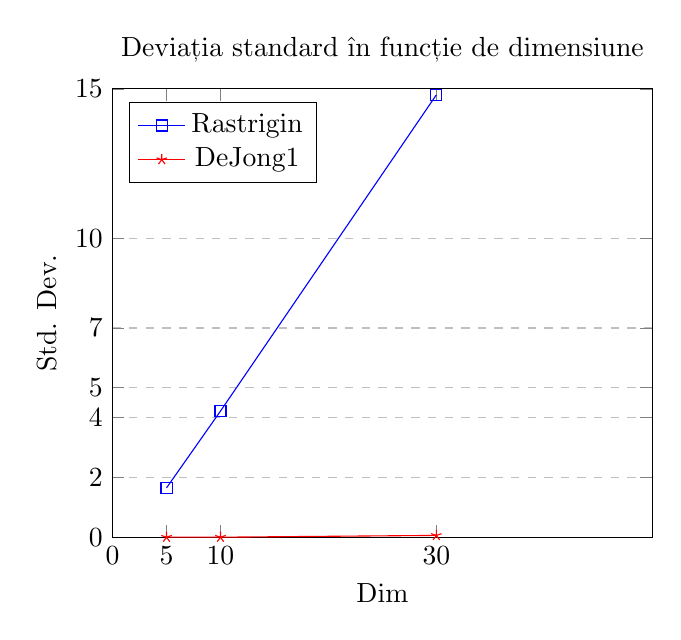
\begin{tikzpicture}
\begin{axis}[
    title={Deviația standard în funcție de dimensiune},
    xlabel={Dim},
    ylabel={Std. Dev.},
    xmin=0, xmax=50,
    ymin=0, ymax=15,
    xtick={0, 5, 10, 30},
    ytick={0, 2, 4, 5, 7, 10, 15},
    legend pos=north west,
    ymajorgrids=true,
    grid style=dashed,
]

\addplot[
    color=blue,
    mark=square,
    ]
    coordinates {
    (5,1.65)(10,4.22)(30,14.80)
    };
 
    
\addplot[
    color=red,
    mark=star,
    ]
    coordinates {
    (5,0.00)(10,0.00)(30,0.06)
    };
    \legend{Rastrigin, DeJong1}
    
    
\end{axis}
\end{tikzpicture}

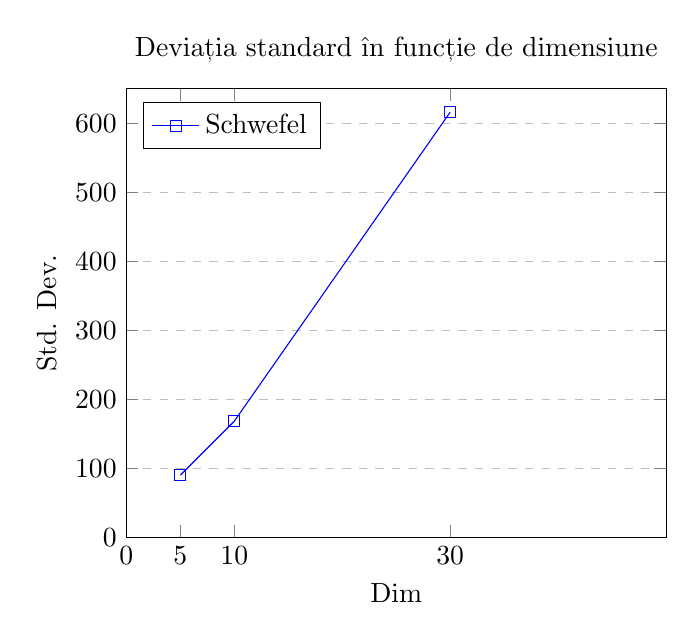
\begin{tikzpicture}
\begin{axis}[
    title={Deviația standard în funcție de dimensiune},
    xlabel={Dim},
    ylabel={Std. Dev.},
    xmin=0, xmax=50,
    ymin=0, ymax=650,
    xtick={0, 5, 10, 30},
    ytick={0, 100, 200, 300, 400, 500, 600, 700},
    legend pos=north west,
    ymajorgrids=true,
    grid style=dashed,
]

\addplot[
    color=blue,
    mark=square,
    ]
    coordinates {
    (5,90.00)(10,168.25)(30,616.23)
    };
    \legend{Schwefel}
    
    
\end{axis}
\end{tikzpicture}

\subsection{Interpretare}
\subsubsection{5 dimensiuni}
Toate cele 4 metode produc soluții asemănătoare. Simulated Annealing are cea mai slabă soluție în cazul funcției lui Rastrigin.\\
În ceea ce privește timpul de execuție HC First Improvment și SA au timpi foarte mici, fiind urmați de HC Best Improvment, și de GA cu un timp de aproape 4 ori mai mare (excepție făcând Schwefel pentru care GA și HC Best Improvment sunt asemănători).\\
Din punct de vedere al deviației standard, SA are o valoare de aproape 4 ori mai mare în cazul funcției Schwefel.\\


\subsubsection{10 dimensiuni}
HC Best Improvment continua să ofere cele mai apropiate soluții de cele reale, însă timpul de execuție este substanțial mai mare.(109.499 secunde în cazul funcției Schwefel).\\
HC First Improvment și SA ofera rezultate identice pentru minimul funcțiilor Rastrigin și Michalewicz (și foarte apropiate pentru DeJong) însa diferă observabil la rezultatul mediu în cazul funcției Rastrigin.\\
GA ajunge pe locul 3 ca timp de execuție, iar în cazul funcției lui Schwefel oferă un rezultat foarte apropiat de cel al HC Best Improvment dar într-un timp de 5 ori mai mic.
SA și GA au cele mai mari deviații standard.\\  


\subsubsection{30 dimensiuni}
Toate cele 4 metode încep să produca rezultate departate față de cele reale. GA este pe primul loc, urmată de SA. HC Best Improvment nu poate fi luat în calcul la aceasta categorie datorită monstrei statistice foarte mici.\\
HC First Improvment și SA au în continuare timpii asemanatori de execuție, excepție făcând funcția Schwefel, pentru care HC are un timp dublu.\\
HC Best Improvment are un timp de execuție uriaș, în comparație cu celelate doua metode. În cazul funcției Schwefel o singura rulare a algoritmului a durat 2942.72 secunde, de aici și alegerea unei monstre statistice foarte mici.\\
Se observă ca SA are o deviație standard mult mai mare decât HC First Improvment.\\
GA are cele mai slabe rezultate și ce mai mare deviație standard dintre cele 4 metode, însă ca timp de execuție se situează pe o poziție medie.


\section{Concluzii}
\textbf{Pentru dimensiunea 5}, toate metodele au returnat o valoare apropiată de cea reală. Deci toate 4 sunt metode bune pentru determinarea minimului.\\
\textbf{Pentru dimensiunea 10}, HC First Improvment și SA încep să se îndepărteze ușor de rezultatele reale, în timp HC Best Improvment oferă cele mai bune raspunsuri, dar cu prețul unui timp mai mare. \\
GA oferă soluții suficient de bune pentru DeJong și Schwefel într-un timp mult mai bun decât BIHC.\\
\textbf{Pentru dimensiunea 30}, HC Best Improvment devine inutil de executat datorita timpului uriaș, în schimb SA reușește sa producă cele mai bune rezultate și cei mai buni timpi. GA rămâne pe poziția 3 ca timp de execuție, dar oferă cele mai slabe soluții. Asadar, SA devine metoda recomandată pentru dimensiuni mari ale funcției.


\begin{thebibliography}{9}

\bibitem{Maxim și minim}
  Minim și maxim\\
  \url{https://en.wikipedia.org/wiki/Maxima_and_minima}

\bibitem{HC și SA}
  Hill Climbing și Simulated Annealing\\
  \url{https://profs.info.uaic.ro/~eugennc/teaching/ga/}\\
  \url{http://www.lia.deis.unibo.it/~aro/pubs/blum_roli_metaheuristics-preprint.pdf}
  
\bibitem{Intocmirea raportului}
  \begin{flushleft}
  Intocmirea unui raport \\ Formularea introducerii.
  \url{https://www.monash.edu/rlo/assignment-samples/engineering/eng-writing-technical-reports/introduction}
  \end{flushleft}
  
\bibitem{Hill Climbing}
  Tipuri de Hill Climbing\\
  \url{https://www.geeksforgeeks.org/introduction-hill-climbing-artificial-intelligence/}
  
\bibitem{SA}
  Simulatin Annealing\\
  \url{http://www.cs.cmu.edu/afs/cs.cmu.edu/project/learn-43/lib/photoz/.g/web/glossary/anneal.html}
  
\bibitem{Algoritm genetic}
  Algoritm genetic\\
  \url{https://www.geeksforgeeks.org/genetic-algorithms/}\\
  \url{http://www.lendek.net/teaching/opt_en/ga.pdf}
  
 \bibitem{De Jong1}
  De Jong1\\
  \url{http://www.geatbx.com/docu/fcnindex-01.html#P89_3085}\\
  Grafic\\
\url{https://www.sfu.ca/~ssurjano/spheref.html}
  
\bibitem{Schwefel}
  Schwefel\\
  \url{http://www.geatbx.com/docu/fcnindex-01.html#P150_6749}\\
    Grafic\\
\url{https://www.sfu.ca/~ssurjano/schwef.html}
  
\bibitem{Rastrigin}
  Rastrigin\\
  \url{http://www.geatbx.com/docu/fcnindex-01.html#P140_6155}\\
    Grafic\\
\url{https://www.sfu.ca/~ssurjano/rastr.html}
  
\bibitem{Michalewicz}
  Michalewicz\\
  \url{http://www.geatbx.com/docu/fcnindex-01.html#P204_10395}\\
  \url{http://www.alliot.mobi/papers/gecco2014b.pdf}\\
    Grafic\\
\url{https://www.sfu.ca/~ssurjano/michal.html}
  
  
\end{thebibliography}  
\end{document}